%\providecommand{\main}{..}
%\documentclass[\main/main.tex]{subfiles}


\begin{document}




One important methodological remark is that we decided to compute mortality risk pooling data from all waves 1, 2, 4, 5 and 6 and all countries together. This strategy is likely to introduce some bias as mortality risk may vary over year of interview and over country. However, by looking at period life table from the HMD (see  section \ref{HMD}), we notice that the nine selected countries of this study share very similar mortality patterns. Therefore, we believe that this inaccuracy is less critical than the fact of estimating prevalence from very small samples. 


We obtain mortality risk for each one-year age class by taking the ratio of people dying at a given age to total individuals in that age class, after conditioning on health condition and gender. Figure \ref{fig:mortality_risk_SHARE_not_disabled} presents the estimates for female and male population in a healthy status. 

\begin{figure}[H]
    \centering \textbf{Mortality risk}\par\medskip
        \centering
        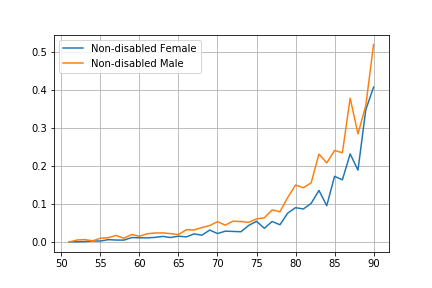
\includegraphics[scale=.5]{images/mortality_regime_SHARE_not_disabled.png}
    \caption{Average probability of dying from age $x$ to $x+1$ for all waves and countries pooled together (healthy individuals). \textit{Source:} SHARE  }
    \label{fig:mortality_risk_SHARE_not_disabled}
\end{figure}

Figure \ref{fig:mortality_risk_SHARE_disabled} presents the estimates for female and male population in a disabled status. 

\begin{figure}[H]
    \centering \textbf{Mortality risk}\par\medskip
        \centering
        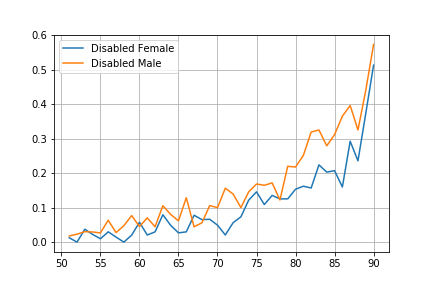
\includegraphics[scale=.5]{images/mortality_regime_SHARE_disabled.png}
    \caption{Average probability of dying from age $x$ to $x+1$ for all waves and countries pooled together (disabled individuals). \textit{Source:} SHARE}
    \label{fig:mortality_risk_SHARE_disabled}
\end{figure}

As we can see, the probability of dying from one year to the next increases with age. However, there is a lot on noise in our estimates probably due to the small sample size. In order to force mortality risk to be monotonically increasing, we decided to fit an exponential function. Figure \ref{fig:mortality_risk_SHARE} describes the fitted mortality risk we obtained.


\begin{figure}[H]
    \centering \textbf{Mortality risk}\par\medskip
        \centering
        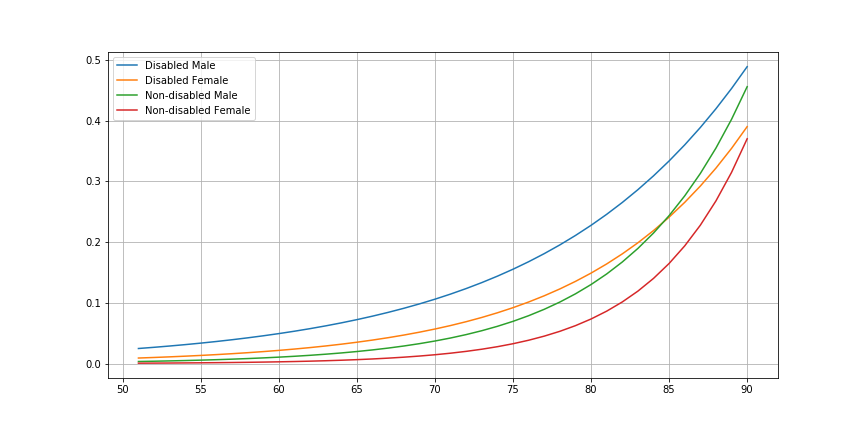
\includegraphics[scale=.5]{images/mortality_regime_SHARE.png}
    \caption{Average probability of dying from age $x$ to $x+1$ for all waves and countries pooled together. \textit{Source:} SHARE}
    \label{fig:mortality_risk_SHARE}
\end{figure}

As expected, the risk of mortality is generally higher for men than for women and for people with disabilities than for healthy ones. 

\end{document}